\documentclass[a4paper, 12pt]{article}

\usepackage[top=2cm, bottom=2cm, left=2.5cm, right=2.5cm]{geometry}
\usepackage[utf8]{inputenc}
\usepackage{amsmath, amsfonts, amssymb}
\usepackage{graphicx} % inserir figuras - \includegraphics[scale=•]{•}
\usepackage{float} % ignorar regras de tipografia e inserir figura aonde queremos.
\usepackage[brazil]{babel} % Trocar Figure para Figura.
\usepackage{indentfirst}
\pagestyle{empty}


\begin{document}
\begin{figure}[H]
	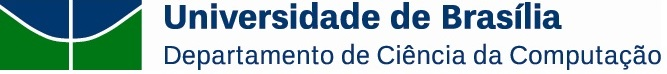
\includegraphics[scale=0.9]{UnB_CiC_Logo.jpg}
\end{figure}
\noindent\rule{\textwidth}{0.4pt}
\begin{center}
	\textbf{{\Large Introdução à Ciência da Computação - 113913}} \newline \newline
	\textbf{{\large Prova 1} \\
	\vspace{9pt}
	{\large Questão A}} \\
	\noindent\rule{\textwidth}{0.4pt}
	\newline
\end{center}

\textbf{{\large Observações:}}
\begin{itemize}
	\item As provas também serão corrigidas por um \textbf{corretor automático}, portanto é necessário que as entradas e saídas do seu programa estejam conforme o padrão especificado em cada questão (exemplo de entrada e saída). Por exemplo, não use mensagens escritas durante o desenvolvimento do seu código como “Informe a primeira entrada”. Estas mensagens não são tratadas pelo corretor, portanto a correção irá resultar em resposta errada, mesmo que seu código esteja correto.
	\item Serão testadas várias entradas além das que foram dadas como exemplo, assim como as listas.
	\item Assim como as listas, as provas devem ser feitas na versão Python 3 ou superior.
	\item Leia com atenção e faça \textbf{exatamente} o que está sendo pedido.
\end{itemize}
\newpage % Questão A 
\begin{center}
\textbf{{\Large Questão A - Despoluição em bacias hidrográficas}}
\end{center}
\vspace{5pt}
Bacia Hidrográfica é a área ou região de drenagem de um rio principal e seus afluentes. É a porção do espaço em que as águas das chuvas, das montanhas, subterrâneas ou de outros rios escoam em direção a um determinado curso d’água, abastecendo-o. Os serviços de saneamento devem ser analisados pela perspectiva da Bacia Hidrográfica (BH).  Muitos municípios brasileiros não possuem tratamento de esgotos adequado ou sequer disponibilizam o serviço para sua população. O lançamento desses efluentes nos corpos hídricos comprometem a qualidade e os usos das águas, causando implicações danosas à saúde pública e ao equilíbrio do meio ambiente. Quanto maior a Demanda Biológica por Oxigênio (DBO) mais poluído está o efluente. 
\newline \newline
\textbf{{\large Entrada}} \newline
A primeira linha contém um inteiro N que irá indicar quantas entradas o programa deve receber.
\newline
Em seguida serão fornecidas N linhas, cada linha com os seguintes dados do município: Nome, população urbana (inteiro), vazão de efluente sem coleta e sem tratamento em L/s (float), DBO no efluente sem coleta e sem tratamento em KgDBO/dia (float), a população atendida por sistema de coleta e tratamento de esgoto (inteiro).
\newline \newline
\textbf{{\large Saída}} \newline
Nome do município que apresenta a maior vazão de esgoto sem tratamento.
\newline
Nome do município com a menor DBO no efluente.
\newline
A taxa média percentual da população urbana não atendida com esgoto sanitário com precisão de 2 casas decimais.
\begin{table}[H]
\centering
\begin{tabular}{|1|1|}
\hline
\textbf{Exemplo de Entrada} & \textbf{Exemplo de Saída} \\ \hline
4       &   
\\
Ariquemes-RO 85770 125.7 2.8 2000  & Ji-Parana-RO
\\
Cabixi-RO 2771 4.3 0.0 0            & Cabixi-RO
\\
Ji-Parana-RO 115123 145.0 8.0 115123  & 11.23
\\
Cajubim-RO 13520 19.5 0.2  13000 &   
\\ \hline
\end{tabular}
\caption{Questão A}
\end{table}
\flushright
\textbf{\Large Boa Prova!}
\end{document}